\section{Method}
This lab is broken up into 6 parts, the first four of which deal with the spectral lines of gases, and the last two of which deal with the spectrums of differently dyed solutions.

Figure \ref{fig:gas_setup} shows the setup for the gas portion of the lab, with a spectral tube connected to a power supply. The clamp stand is used to hold the probe in place above the tubes, and a diffraction grating is used to observe the spectral lines. These lines are displayed on a computer (not shown), and images of the lines and key values are taken for analysis. When measuring peaks, the value is taken at the peak of the line, and the uncertainty is taken as the full width at half height (FWHH) of the line.
\begin{figure}[H]
    \centering
    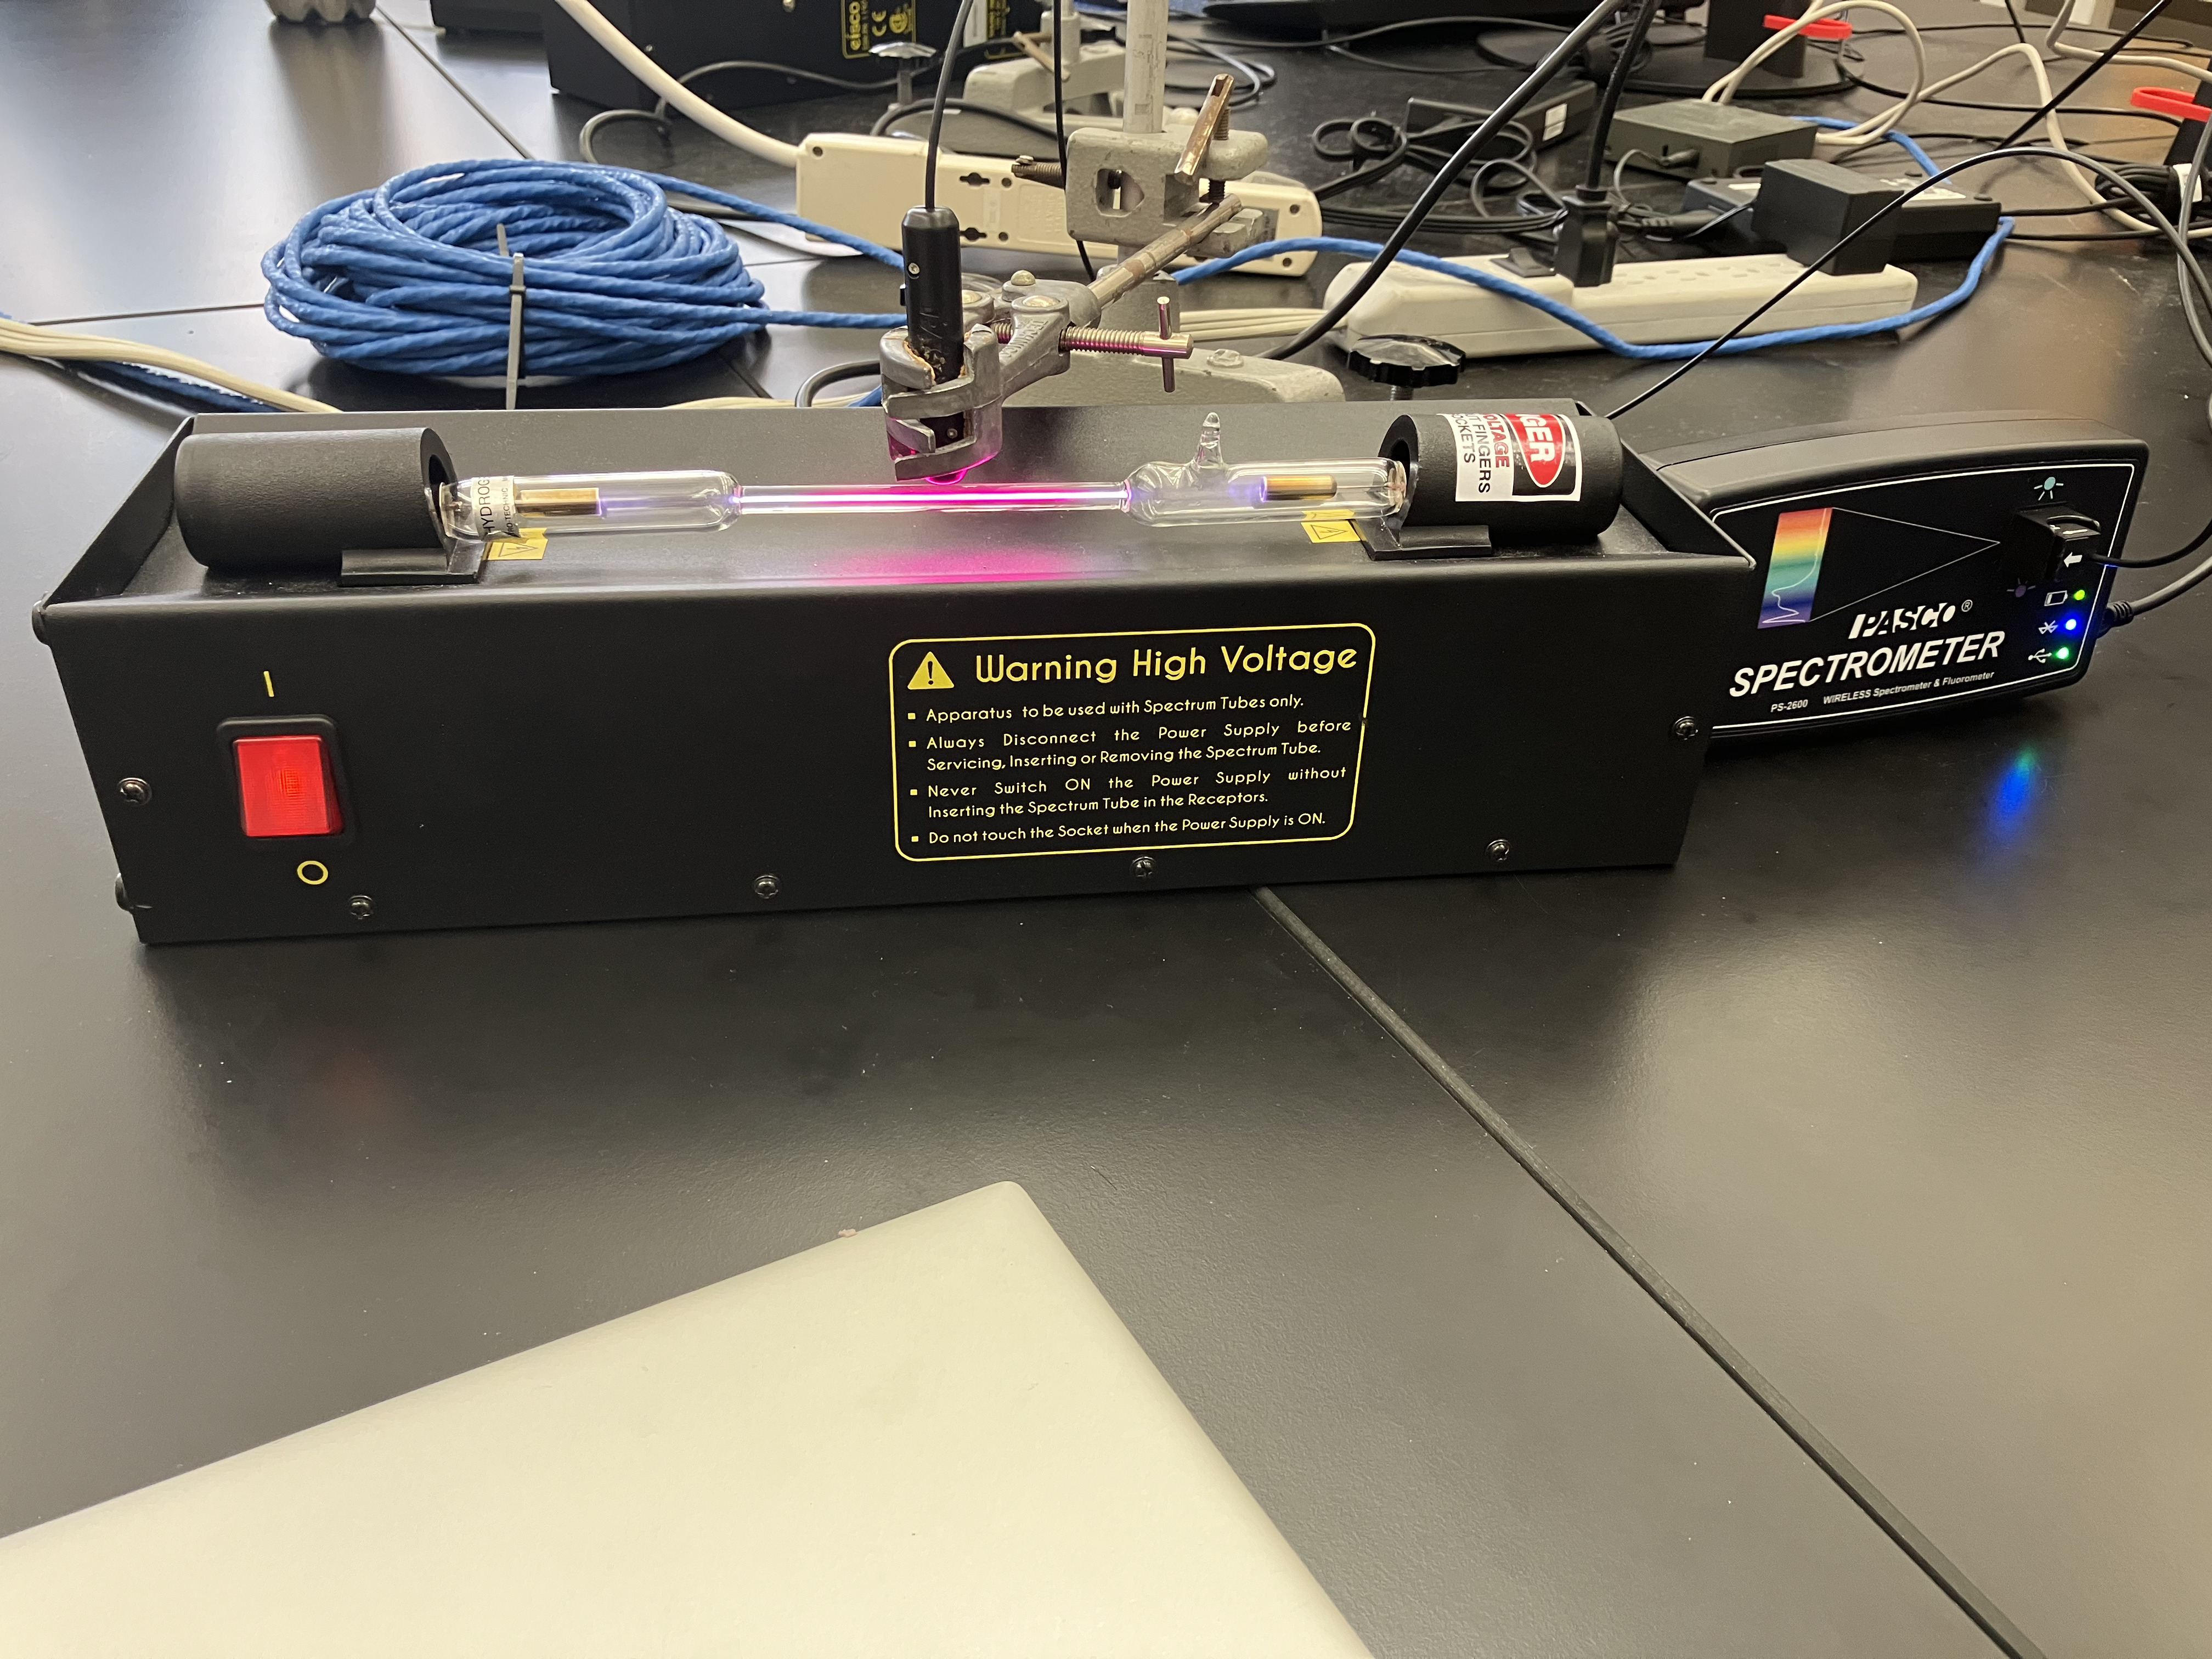
\includegraphics[width=0.8\textwidth]{method/gas_setup.jpg}
    \caption{Setup for the gas portion of the lab.}
    \label{fig:gas_setup}
\end{figure}

Figure \ref{fig:dye_setup} shows the setup for the dyed solutions portion of the lab. The spectrometer is used to measure the absorbance of the solutions by shining a white light through the solution and measuring the intensity of the output light at various wavelengths. 
\begin{figure}[H]
    \centering
    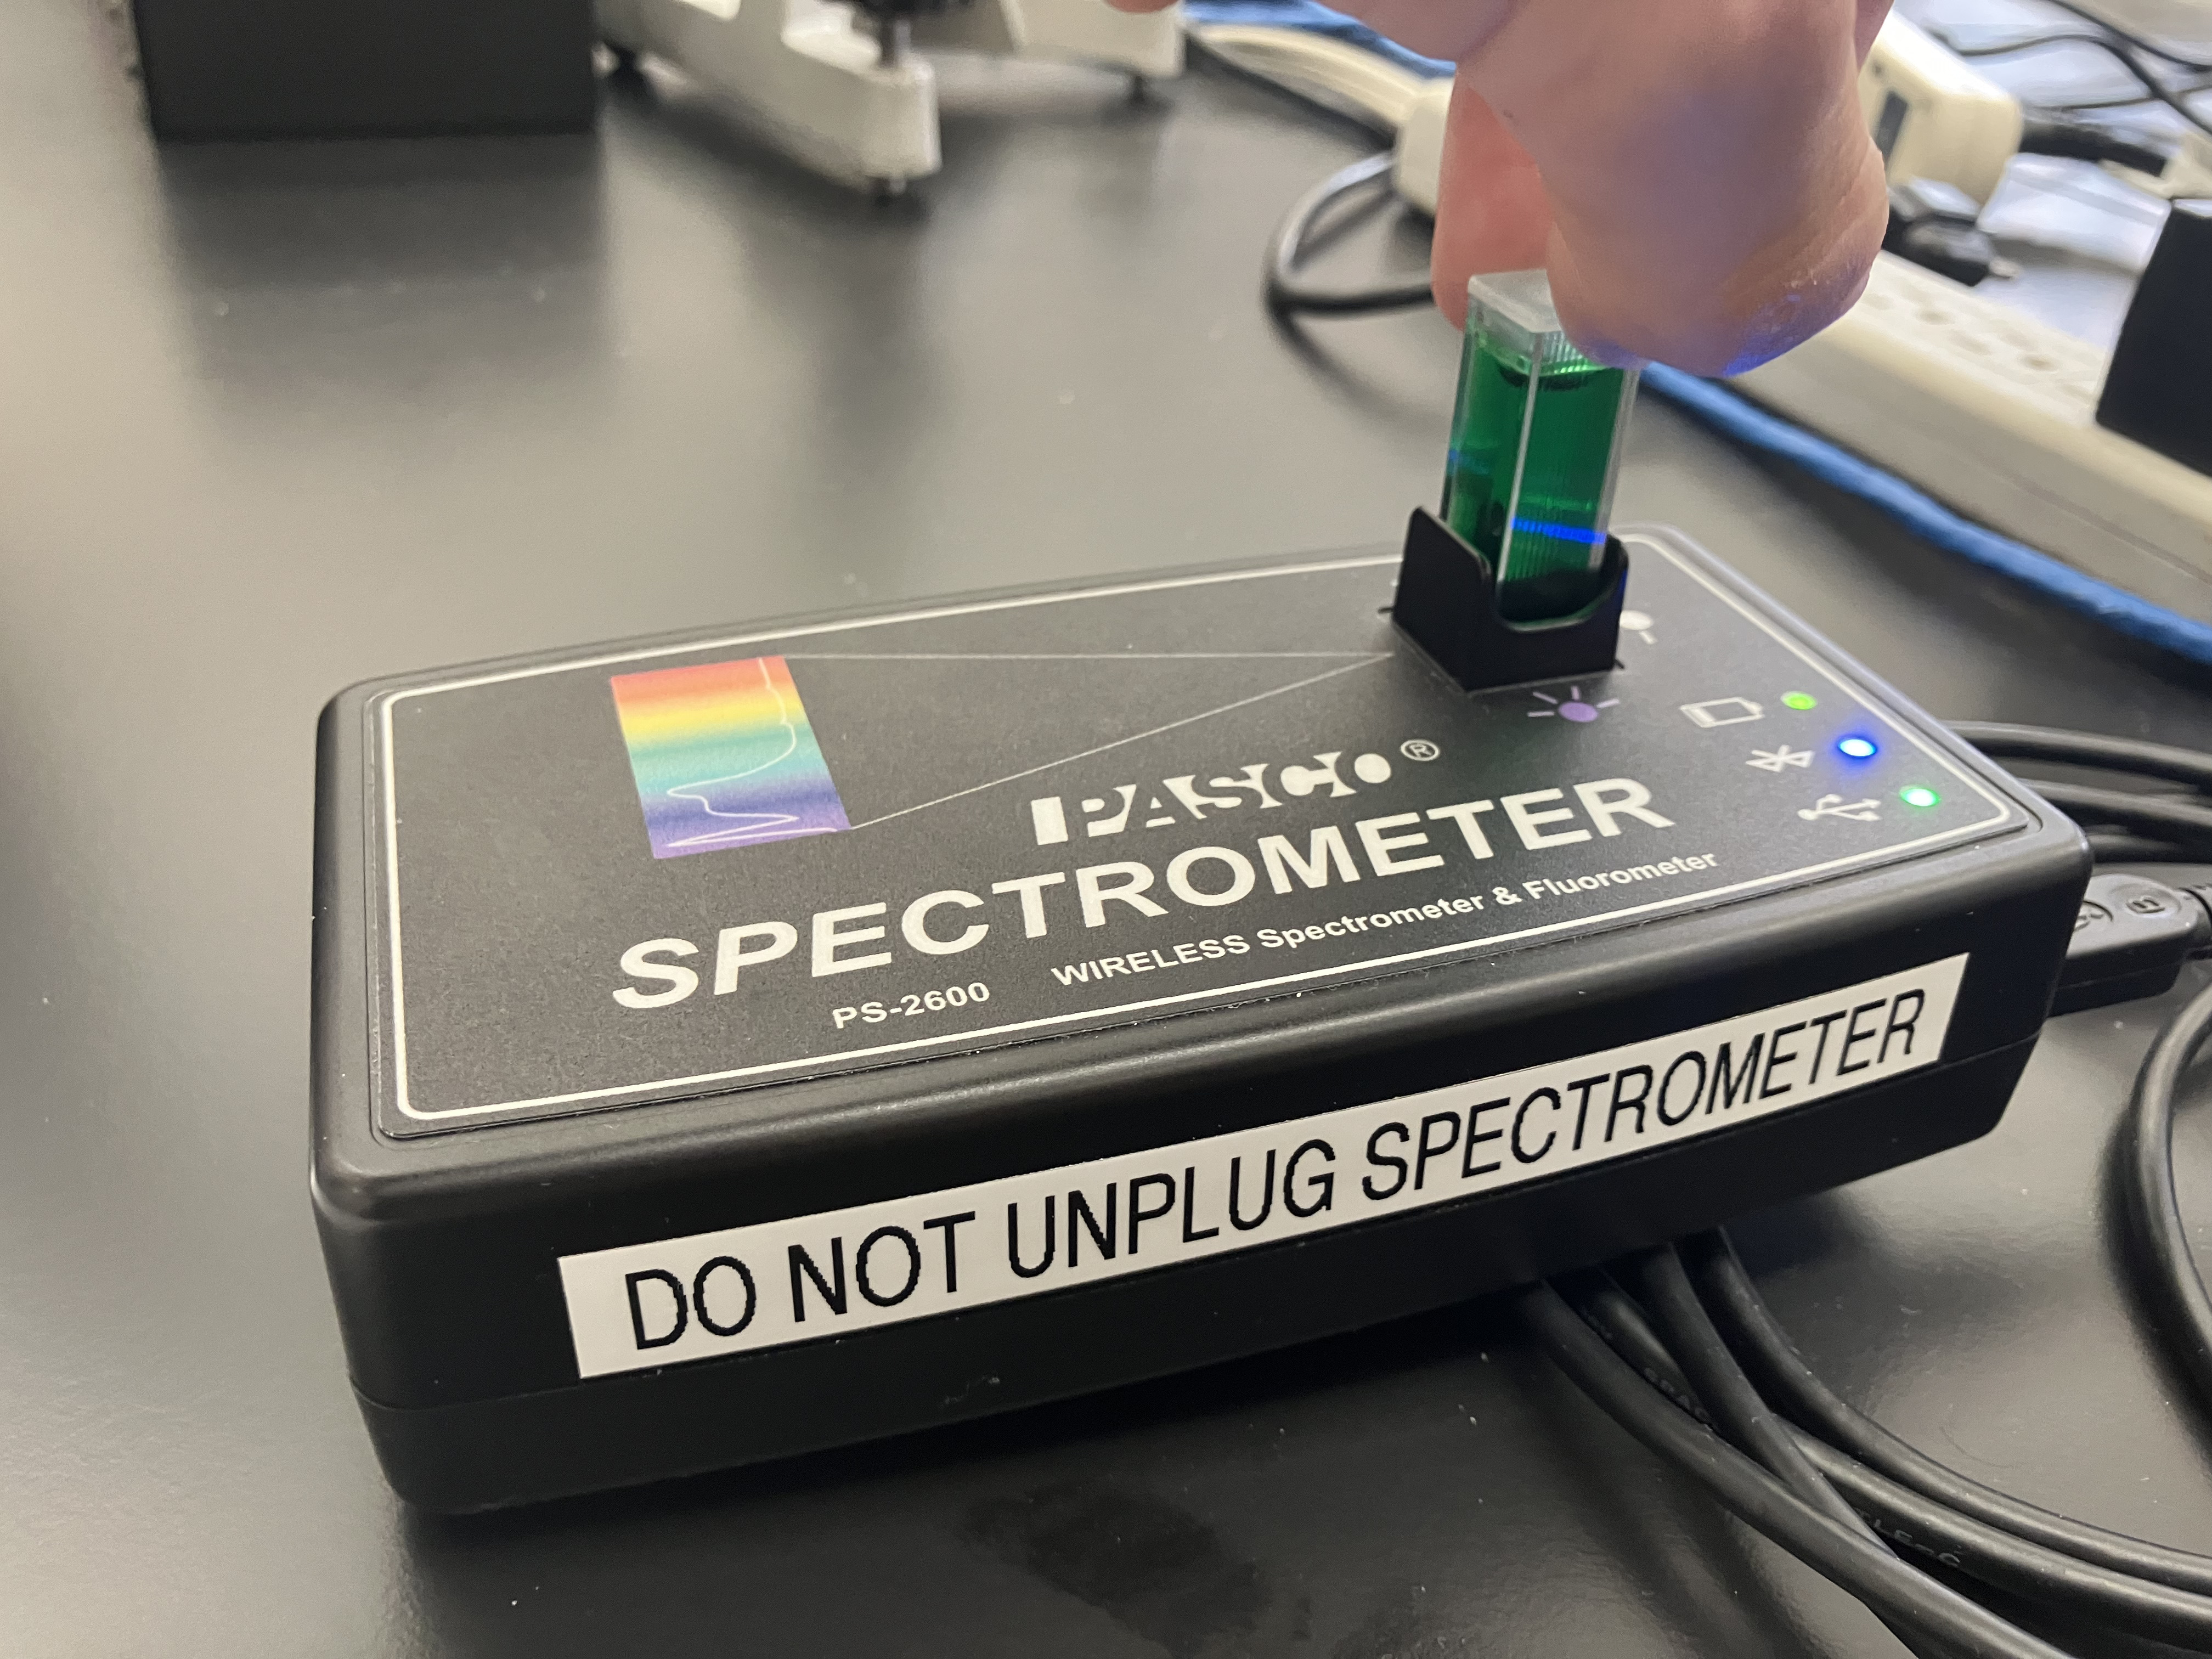
\includegraphics[width=0.8\textwidth]{method/solution_setup.jpg}
    \caption{Setup for the dyed solutions portion of the lab.}
    \label{fig:dye_setup}
\end{figure}

\subsection{Part 1: Mercury}
Using known wavelengths of the mercury spectral lines From \cite{mercury_spectral_lines}, we measure the experimental locations of the peaks and apply a linear regression against the known values to convert the computer output to true wavelengths. We also repeat this process for the photon energies of the lines.

\subsection{Part 2: Hydrogen}
For this section, we again measure the experimental locations of the peaks, but compare them with the expected quantum energy of the Balmer series of hydrogen.

\subsection{Part 3: Helium}
We measure the experimental locations of the peaks.

\subsection{Part 4: Unknown Gas}
Lastly, we measure the experimental locations of the peaks and convert them to true wavelengths using the results from Part 1. We then compare these wavelengths to known spectral lines to identify the gas.

\subsection{Part 5: Transmittance and Absorbance}
We measure the transmittance and absorbance of the blue, green, and red dye solutions at various wavelengths. We then compare the experimental absorbance to the expected absorbance using the formula $A = -log_{10}(T/100)$ and identify 